%!TEX root = ../template.tex
%%%%%%%%%%%%%%%%%%%%%%%%%%%%%%%%%%%%%%%%%%%%%%%%%%%%%%%%%%%%%%%%%%%%
%% chapter3.tex
%% NOVA thesis document file
%%
%% Chapter with a short laext tutorial and examples
%%%%%%%%%%%%%%%%%%%%%%%%%%%%%%%%%%%%%%%%%%%%%%%%%%%%%%%%%%%%%%%%%%%%
\chapter{Inversión para una SD-WAN}
\label{cha:Inversión para una SD-WAN}

\section{Precios en una Red SD-WAN} % (fold)
\label{sec:Precios en una Red SD-WAN}

Una de las mayores motivaciones para el desarrollo de este proyecto es reducir el costo en OPEX que costarían los enlaces de los proveedores de servicio al trasladar los servicios de la empresa a la nube, ya que los costos de ancho de banda se reducirían notablemente al realizar esta migración con SD-WAN \textbf{la tabla 4.1} muestra una comparación aproximada de los costos de los enlaces WAN requeridos con y sin SD-WAN. 
\\
\\
Dichos costos son calculados tomando en cuenta los valores publicados por google para su aplicación de Gsuite, ya que el cliente entre otras cosas realizará reuniones a través de Google Meet, esto requiere 3.2MB de ancho de banda por participante.

\begin{table}[ht]
	\caption{Tabla de Precios  para la Implementación de una SW-WAN.}
	\label{tab:hla:results}
\centering
\begin{tabular}{lccccc}
	\toprule
	\multicolumn{1}{c}{\textbf{Tipo de Oficina}} 	& \textbf{Tienda}	& \textbf{Regional}	& \textbf{Oficina Regional}\\
	\midrule
\cite{Usuarios}~Promedio 		& 3 & 25 & 60	 \\
\cite{Sesiones}~de Video Simultáneas & 1& 8	& 20	\\
\cite{Trafico}~de Datos	& 5MB	& 10MB	& 20MB	\\
\cite{BW}~Servicio Actual		& 10& 7	& 14	 \\
\cite{BW}~Requerido	& 9MB	& 25MB	& 84MB	 \\
\cite{Costo}~Actual			& 221741	& 1260741	& 1803563	\\
\cite{Costo}~Mensual Red Legacy		& 221741	& 3607126	& 6782000 \\
\cite{Costo}~Mensual SD-WAN	& 221741	& 1842102	& 3972361\\
	\midrule
	\textbf{Total}			& \textbf{--}		& \textbf{--}		& \textbf{--} \\
	\bottomrule
\end{tabular}
\end{table}
Adicional al costo de los enlaces, el OPEX también se vería reducido al requerir menor tiempo de los recursos de IT en la administración de la red, ya que al automatizar las configuraciones y cambios la velocidad de aprovisionamiento se vería ampliamente mejorada y por tanto su costo sería menor.


\section{Costos para Implementación en Infraestructura Cloud} % (fold)
\label{sec:Costos para Implementación en Infraestructura Cloud}


\subsection{Amazon}

\textcolor{blue}{Amazon:} multinacional de comercio electrónico y servicios de computación en la nube, contiene cuatro modelos para compra de instancias en Cloud conocido como Amazon EC2.

\begin{itemize}
\item[•] \textbf{Baja Demanda:} \textit{"Con las instancias bajo demanda, paga por la capacidad informática por hora o por segundo, según las instancias que use. Ya no serán necesarios los contratos a largo plazo ni los pagos iniciales. Puede aumentar o reducir la capacidad informática en función de las exigencias de su aplicación y pagar únicamente la tarifa por hora específica de la instancia que use." En la \textbf{tabla 4.1} se observa algunos costos de baja demanda.}

\begin{table}[ht]
	\caption{Amazon EC2 Pricing.}
	\label{tab:hla:results}
\centering
\begin{tabular}{lccccc}
	\toprule
	\multicolumn{1}{c}{\textbf{vCPU}} 	& \textbf{ECU}	& \textbf{Memory (GiB)}	& \textbf{Instance Storage (GB)}
	& \textbf{Linux/UNIX Usage}\\
	\midrule
\cite{a1.medium}~1 		& N/A & 2GiB & EBS Only	& \$0.0255 per Hour \\
\cite{a1.large}~2 		& N/A & 4GiB & EBS Only & \$0.051 per Hour	\\
\cite{a1.xlarge}~4		& N/A & 4GiB & EBS Only & \$0.051 per Hour	\\
\cite{a1.2xlarge}~8 	& N/A & 16GiB & EBS Only & \$0.204 per Hour	\\
\cite{a1.4xlarge}~16	& N/A & 32GiB & EBS Only & \$0.408 per Hour	\\
\cite{t3.nano}~2		& N/A & 0.5GiB & EBS Only & \$0.0052 per Hour	\\
\cite{t3.micro}~2   	& N/A & 1GiB & EBS Only & \$0.0104 per Hour	\\
	\midrule
	\textbf{Total}			& \textbf{--}		& \textbf{--}		& \textbf{--} \\
	\bottomrule
\end{tabular}
\end{table}

\item[•] \textbf{Instancias Reservadas:}\textit{Las instancias reservadas ofrecen un descuento importante (de hasta el 75 \%) en comparación con los precios de las instancias bajo demanda. Además, cuando se asignan instancias reservadas a una zona de disponibilidad específica, se proporciona una reserva de capacidad, lo que le aporta más tranquilidad en relación con la posibilidad de lanzar instancias cuando las necesite.
\\
\\
Para las aplicaciones con estado constante o uso previsible, las instancias reservadas pueden suponer un ahorro considerable en comparación con las instancias bajo demanda. Consulte Cómo adquirir instancias reservadas para obtener más información.}
\item[•] \textbf{Instancias de Spot:} \textit{Las instancias de spot de Amazon EC2 le permiten solicitar capacidad informática sobrante de Amazon EC2 con descuentos de hasta el 90\% en comparación con el precio de las instancias bajo demanda.}
\item[•] \textbf{Host Dedicados:}\textit{Un host dedicado es un servidor físico de EC2 exclusivo para su uso. Los hosts dedicados pueden ayudarle a reducir costos porque le permiten usar sus licencias existentes de software enlazado al servidor, incluidos Windows Server, SQL Server y SUSE Linux Enterprise Server (en función de los términos de su licencia). También pueden ayudarle a cumplir requisitos de conformidad.}


\begin{table}[ht]
	\caption{On-Demand Pricing.}
	\label{tab:hla:results}
\centering
\begin{tabular}{lccccc}
	\toprule
	\multicolumn{1}{c}{\textbf{General purpose}} 	& \textbf{Price Per Hour}\\
	\midrule
\cite{a1} 		& \$0.449\\
\cite{m5} 		& \$5.069\\
\cite{m5d}		& \$5.966\\
\cite{m4} 		& \$2.42\\

	\midrule
	\textbf{Total}			& \textbf{--}	\\
	\bottomrule
\end{tabular}
\end{table}


\end{itemize}

Donde se puede implementar infraestructura de telecomuicaciones a un bajo costo, contando con todos los servicios necesarios de una red.
\subsection{Microsoft Azure}

\textcolor{blue}{Azure:} es en constante expansión de servicios en la nube para ayudar a su organización a sastifacer sus necesidades comerciales. Le otorga la libertad de crear, administrar e implementar aplicaciones en una red mundial.

Para máquinas virtuales tenemos la siguiente \textbf{figura 4.1 Costo con Azure}

\begin{figure}[htbp]
  \centering
  %\subcaptionbox{\label{fig:leftsubfig}}%
    {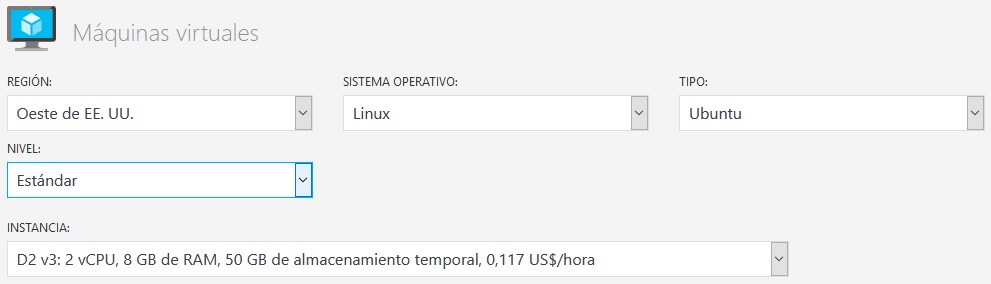
\includegraphics[width=1.0\linewidth]{figure2}}%
%  \subcaptionbox{Another sub-figure\label{fig:rightsubfig}}%
%    {
\includegraphics[width=0.5\linewidth]{knitting-vectorial}}%
  \caption{Precio en Máquinas Virtuales en Azure}
  \label{fig:fig2subfig}
\end{figure}
Para redes virtuales tenemos la \textbf{figura 4.2 Redes Virtuales en Azure}
\begin{figure}[htbp]
  \centering
  %\subcaptionbox{\label{fig:leftsubfig}}%
    {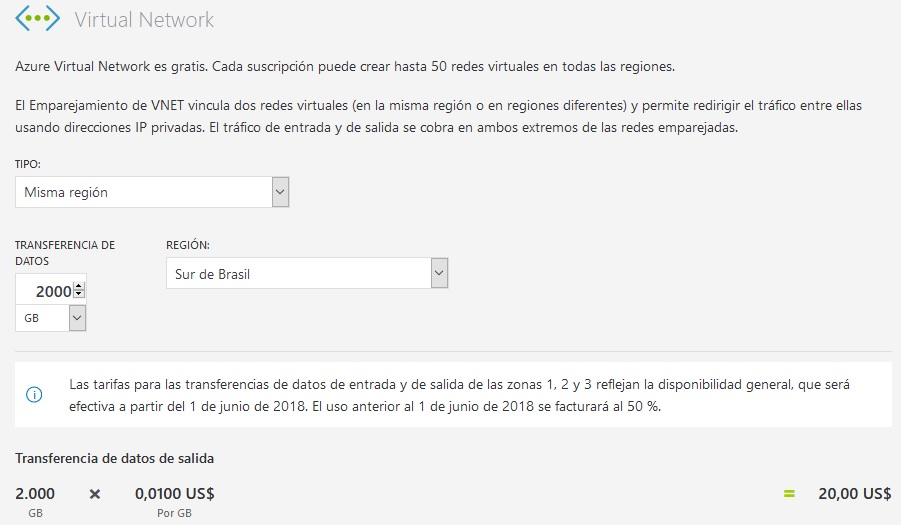
\includegraphics[width=1.0\linewidth]{figure3}}%
%  \subcaptionbox{Another sub-figure\label{fig:rightsubfig}}%
%    {
\includegraphics[width=0.5\linewidth]{knitting-vectorial}}%
  \caption{Precio en Redes Virtuales en Azure}
  \label{fig:fig2subfig}
\end{figure}
%
\\
Podemos encontrar diferentes características, que se requiere en una infraestructura de telecomunicaciones 
Inicie sesión para ver cotizaciones  \textbf{figura 4.3 Infraestructura en Azure}.

*El costo estimado total se basa en los precios aplicables en el día en que se creó la estimación. El costo estimado total real puede variar. Vuelva a abrir el costo estimado para ver el importe total con los precios más recientes
\\
\begin{figure}[htbp]
  \centering
  %\subcaptionbox{\label{fig:leftsubfig}}%
    {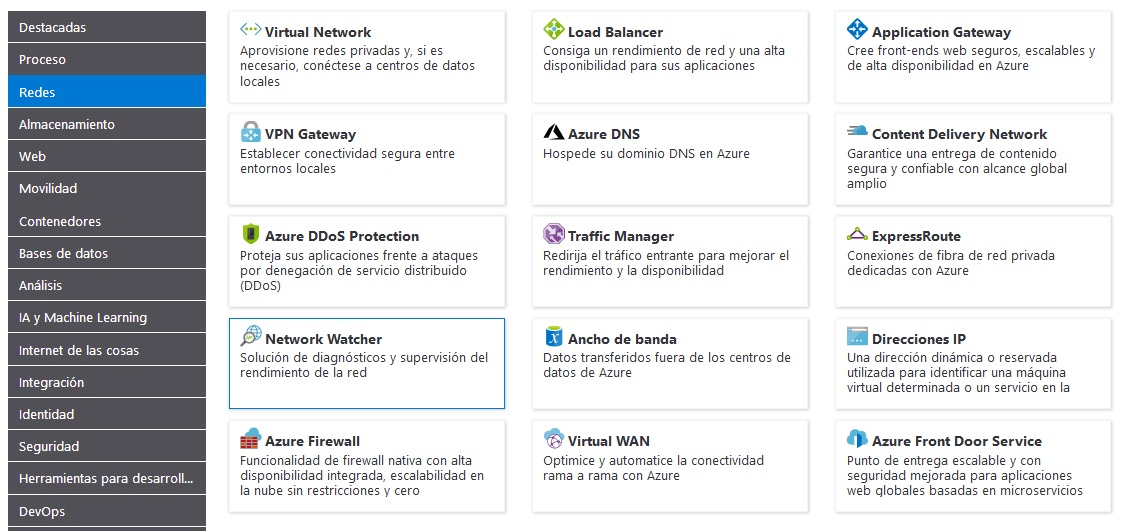
\includegraphics[width=1.0\linewidth]{figure4}}%
%  \subcaptionbox{Another sub-figure\label{fig:rightsubfig}}%
%    {
\includegraphics[width=0.5\linewidth]{knitting-vectorial}}%
  \caption{Diferentes características en Azure para Telecomunicaciones}
  \label{fig:fig2subfig}
\end{figure}

\subsection{Google Cloud}

\textcolor{blue}{Google Cloud:} es una plataforma que ha asociado todas las aplicaciones de desarrollo web que Google 
estaba ofreciendo por separado.
\\
Al adjuntar más servicios en un solo contenedor se desarrolla un fácil administración de los diferentes elementos como almacenamiento, redes, entre otros.

Con Google Cloud se implemento distintos Router para el área diseño de la presente tésis. Los Router que se pudo llegar a implementar fue de la propiedad Cisco el Router CSR 1000v.
\\
Para Google Cloud se puede realizar una estimación de precios en diferentes áreas del mundo ejemplo observamos la \textbf{figura 4.4 Plataform Pricing Calculator}.

\begin{figure}[htbp]
  \centering
  %\subcaptionbox{Producto \label{fig:leftsubfig}}%
  %  {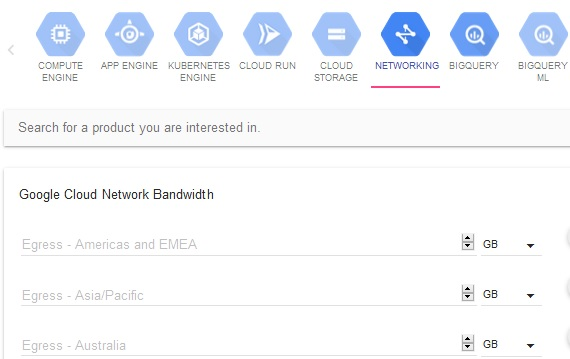
\includegraphics[width=0.4\linewidth]{figure5}}%
 % \subcaptionbox{Estimación\label{fig:rightsubfig}}%
  {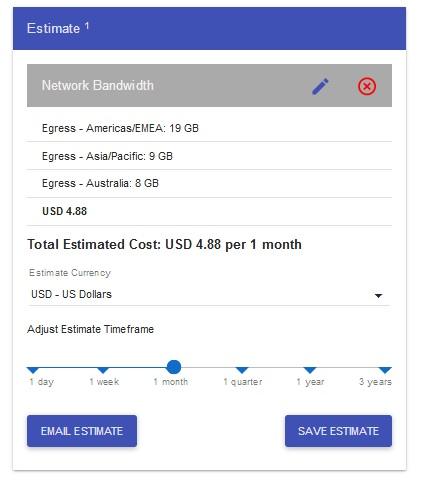
\includegraphics[width=0.8\linewidth]{figure6}}%
  \caption{Plataform Pricing Calculator Google}
  \label{fig:fig2subfig}
\end{figure}

\subsection{Oracle Cloud}

\textcolor{blue}{Oracle:} uno de los más grandes en Base de Datos que enfreta una competencia con IBM desde hace algunos años tiene en sus filas la implementación de Cloud fortaleciendo con grandes herramientas de sistemas opertativos como Linux, también presenta una infratestructura robusta, para instanciar las diferentes máquinas virtuales para nuestro diseño. En la siguiente \textbf{tabla 4.1 Precios Oracle} se detalla la implementación de un Computador con caracteríticas para una empresa entre 100 a 200 empleados.

\begin{table}[ht]
	\caption{Dedicated Compute Classic.}
	\label{tab:hla:results}
\centering
\begin{tabular}{lccccc}
	\toprule
	\multicolumn{1}{c}{\textbf{Product}} 	& \textbf{Price} & \textbf{Metric}\\
	\midrule
\cite{Compute Classic - Model 500} 		& USD \$50,000.00 & 500 OCPUs Month\\
\cite{Compute Classic - Model 1000} 		& USD \$81,000.00 & 1000 OCPUs Month\\
\cite{Compute Classic - Model 1500} 		& USD \$114,000.00 & 1500 OCPUs Month\\
\cite{Compute Classic - Model 2000} 		& USD \$148,000.00 & 2000 OCPUs Month\\

	\midrule
%	\textbf{Total}			& \textbf{--}	\\
	\bottomrule
\end{tabular}
\end{table}

\section{Análisis de Inversión para Cloud} % (fold)
\label{sec:Análisis de Inversión para Cloud}

\subsection{Enfoque al Cliente: Costo, Confiabilidad, Seguridad}
\label{sec:Enfoque al cliente: costo, confiabilidad, seguridad}

Un resumen de investigación de SDxCentral, SD-WAN seguro se ubica entre las tres principales en cuanto a capacidades clave de una red.
El objetivo principal de SD-WAN La tecnología WAN consiste en ofrecer una conexión WAN en la nube, segura y simple, de clase empresarial, con la mayor cantidad de tecnología abierta y basada en software.
Esto se puede usarse para brindar conectividad WAN básica, opara servicios empresariales de primera calidad como VPN, optimización de WAN y control de entrega de aplicaciones (ADC).
\\
\\
Muchas nuevas empresas buscan el potencial en el mercado de WAN definido por software, y las empresas establecidas también están persiguiendo el mercado. Según el IDC, el mercado SD-WAN crecerá a una tasa de crecimiento anual compuesta de 40.4 \% de 2017 a 2022 para llegar a \$ 4.5 mil millones”.
\\
\\
Gartner identifica a los jugadores clave en la tecnología SD-WAN en su Cuadrante Mágico de 2018 para el Informe de Infraestructura de Borde WAN. Nombró a tres líderes: Silver Peak, Cisco y VMware. La firma también reconoció que Riverbed, Citrix, Fortinet, Aryaka y Huawei también son fuertes competidores en el mercado.
\\
\\
Muchos de estos proveedores tienen enfoques del mercado ligeramente diferentes. Por ejemplo, Silver Peak se enfoca en acelerar las aplicaciones de "Software-as-a-Service" (SaaS) en la nube. VMware integró el producto VeloCloud en su propia línea de productos, el VMware NSX SD-WAN de VeloCloud, después de que adquirió VeloCloud
en diciembre de 2017.
\\
\\
El producto contiene aplicaciones de vanguardia, orquestación y puertas de enlace residentes en la nube. Aryaka construyó una red global para que las empresas puedan usar WAN como una red como servicio (NaaS) en cualquier lugar, incluso fuera del área de uno de los puntos de presencia (POP) de Aryaka.
\\
\\
Los proveedores incumbentes de tecnología WAN, como Cisco y Riverbed, que fabrican dispositivos especializados para la conectividad WAN, ahora se centran más en la optimización de WAN y en las ofertas WAN de vanguardia.
Espere que la tendencia se acelere en los próximos años. Lo que comenzó como una
solución para conectividad WAN de sucursales y centros de datos que requieren menos equipos patentados parece expandirse a una amplia gama de ofertas y tecnologías SD-WAN (SDWAN) que incluyen VPN, seguridad, ventaja, optimización de WAN, NaaS y Control de políticas de aplicación.
\\
\\
Si está considerando si SD-WAN mejorará la red de área amplia de su empresa, se ha aprendido que es importante conocer primero las diferentes arquitecturas de SD-WAN.
Como un proveedor de servicios de Internet (ISP) y profesional en este campo  de la nube desde hace
mucho tiempo, he tenido el mejor asiento en la casa para ver cómo la locura de SD-WAN toma vuelo. A medida que aparecen docenas de ofertas de productos SD-WAN, tengo el envidiable trabajo de darle sentido a todo.



% section document_structure (end)


%\section{Dealing with Bibliogrpahy} % (fold)
%\label{sec:dealing_with_bibliogrpahy}

% section dealing_with_bibliogrpahy (end)


%\section{Inserting Tables} % (fold)
%\label{sec:inserting_tables}

% section inserting_tables (end)


%\section{Importing Images} % (fold)
%\label{sec:importing_images}

% section importing_images (end)


%\section{Floats, Figures and Captions} % (fold)
%\label{sec:floats_figures_and_captions}




%\begin{figure}[htbp]
%  \centering
 % \subcaptionbox{One sub-figure\label{fig:leftsubfig}}%
  %  {
\includegraphics[width=0.5\linewidth]{knitting-vectorial}}%
  %\subcaptionbox{Another sub-figure\label{fig:rightsubfig}}%
  %  {
\includegraphics[width=0.5\linewidth]{knitting-vectorial}}%
  %\caption{A figure with two sub-figures!}
  %\label{fig:fig2subfig}
%\end{figure}

%\textbf{And this is a small text that references the Figure~\ref{fig:fig2subfig} and its Subfigures~%\ref{fig:leftsubfig} and~\ref{fig:rightsubfig}.}



%\section{Text Formatting} % (fold)
%\label{sec:text_formatting}

% section text_formatting (end)


%\section{Generating PDFs from \LaTeX} % (fold)
%\label{sec:generating_pdfs_from_latex}

%\subsection{Generating PDFs with pdflatex} % (fold)
%\label{ssec:generating_pdfs_with_pdflatex}


%A typical pass for a document with figures, cross-references and a bibliography would be:
%\begin{verbatim}
%$ pdflatex template
%$ bibtex template
%$ pdflatex template
%$ pdflatex template
%\end{verbatim}



%\subsection{Dealing with Images} % (fold)
%\label{sub:dealing_with_images}


%\subsection{Creating Source Files Compatible with both latex and pdflatex} % (fold)
%\label{ssec:creating_source_files_compatible_with_both_latex_and_pdflatex}


%Para incluir listagens de código no seu documento, deverá incluir o pacote %\emph{listings} e depois usar o ambiente \emph{lstlisting}, como exemplificado na Listagem~\ref{lst:HelloWorld}.

%\lstset{language=Java, caption=Hello World, label=lst:HelloWorld}
%\begin{lstlisting}
%/** 
% * The HelloWorldApp class implements an application that
% * simply prints "Hello World!" to standard output.
% */
%class HelloWorldApp {%
 %   public static void main(String[] args) {%
  %      System.out.println("Hello World!"); // Display the string.
   % }
%}
%\end{lstlisting}


